\documentclass[11pt,a4paper]{report}
\usepackage[textwidth=37em,vmargin=30mm]{geometry}
\usepackage{calc,xunicode,amsmath,amssymb,paralist,enumitem,tabu,booktabs,datetime2,xeCJK,xeCJKfntef,listings}
\usepackage{tocloft,fancyhdr,tcolorbox,xcolor,graphicx,eso-pic,xltxtra,xelatexemoji}

\newcommand{\envyear}[0]{2025}
\newcommand{\envdatestr}[0]{2025-10-19}
\newcommand{\envfinaldir}[0]{webdb/2025/20251019/final}

\usepackage[hidelinks]{hyperref}
\hypersetup{
    colorlinks=false,
    pdfpagemode=FullScreen,
    pdftitle={Web Digest - \envdatestr}
}

\setlength{\cftbeforechapskip}{10pt}
\renewcommand{\cftchapfont}{\rmfamily\bfseries\large\raggedright}
\setlength{\cftbeforesecskip}{2pt}
\renewcommand{\cftsecfont}{\sffamily\small\raggedright}

\setdefaultleftmargin{2em}{2em}{1em}{1em}{1em}{1em}

\usepackage{xeCJK,xeCJKfntef}
\xeCJKsetup{PunctStyle=plain,RubberPunctSkip=false,CJKglue=\strut\hskip 0pt plus 0.1em minus 0.05em,CJKecglue=\strut\hskip 0.22em plus 0.2em}
\XeTeXlinebreaklocale "zh"
\XeTeXlinebreakskip = 0pt


\setmainfont{Brygada 1918}
\setromanfont{Brygada 1918}
\setsansfont{IBM Plex Sans}
\setmonofont{JetBrains Mono NL}
\setCJKmainfont{Noto Serif CJK SC}
\setCJKromanfont{Noto Serif CJK SC}
\setCJKsansfont{Noto Sans CJK SC}
\setCJKmonofont{Noto Sans CJK SC}

\setlength{\parindent}{0pt}
\setlength{\parskip}{8pt}
\linespread{1.15}

\lstset{
	basicstyle=\ttfamily\footnotesize,
	numbersep=5pt,
	backgroundcolor=\color{black!5},
	showspaces=false,
	showstringspaces=false,
	showtabs=false,
	tabsize=2,
	captionpos=b,
	breaklines=true,
	breakatwhitespace=true,
	breakautoindent=true,
	linewidth=\textwidth
}






\newcommand{\coverpic}[2]{
    % argv: itemurl, authorname
    Cover photo by #2~~(\href{#1}{#1})
}
\newcommand{\makeheader}[0]{
    \begin{titlepage}
        % \newgeometry{hmargin=15mm,tmargin=21mm,bmargin=12mm}
        \begin{center}
            
            \rmfamily\scshape
            \fontspec{BaskervilleF}
            \fontspec{Old Standard}
            \fontsize{59pt}{70pt}\selectfont
            WEB\hfill DIGEST
            
            \vfill
            % \vskip 30pt
            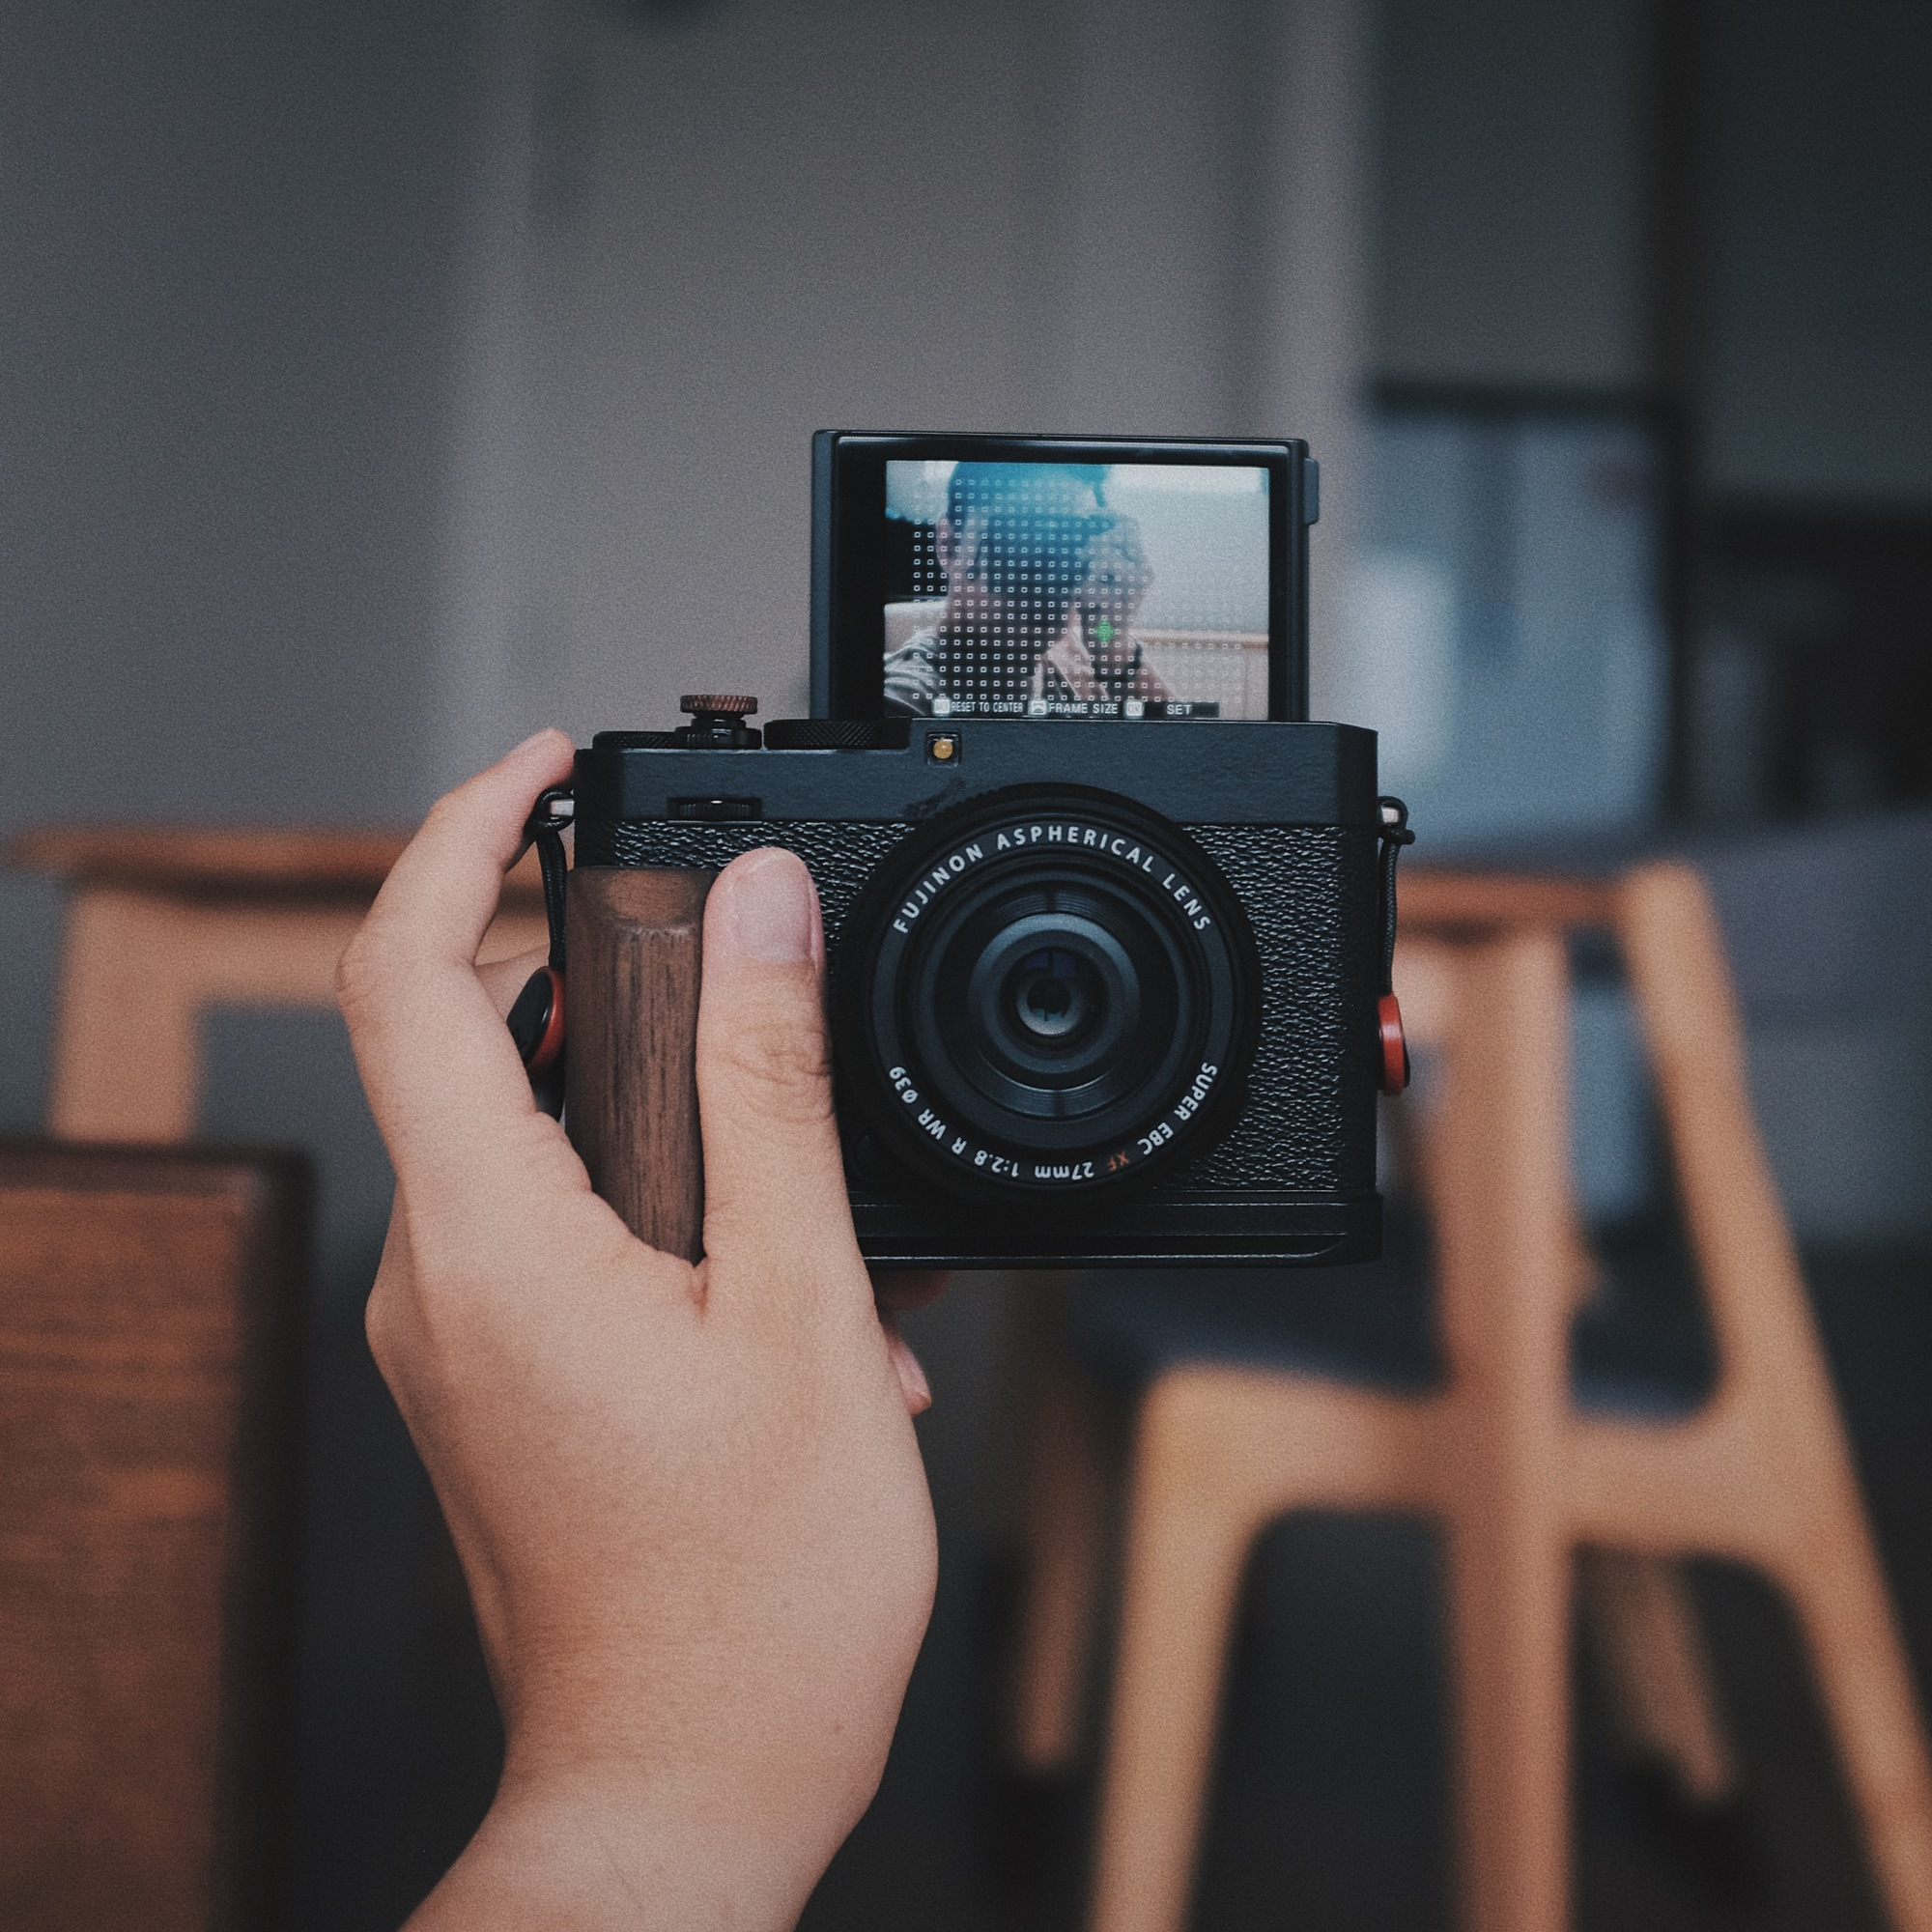
\includegraphics[width=\linewidth]{\envfinaldir/coverpic-prod.jpg}\par
            % \vskip 30pt
            \vfill

            \normalsize\rmfamily\scshape
            \copyright{} The Web Digest Project \hfill\large \envdatestr
        \end{center}
    \end{titlepage}
    % \restoregeometry
}
\newcommand{\simplehref}[1]{%
    \textcolor{blue!80!green}{\href{#1}{#1}}%
}
\renewcommand{\contentsname}{\center\Huge\sffamily\bfseries Contents\par\vskip 20pt}
\newcounter{ipartcounter}
\setcounter{ipartcounter}{0}
\newcommand{\ipart}[1]{
    % \vskip 20pt
    \clearpage
    \stepcounter{ipartcounter}
    \phantomsection
    \addcontentsline{toc}{chapter}{#1}
    % \begin{center}
    %     \Huge
    %     \sffamily\bfseries
    %     #1
    % \end{center}
    % \vskip 20pt plus 7pt
}
\newcounter{ichaptercounter}
\setcounter{ichaptercounter}{0}
\newcommand{\ichapter}[1]{
    % \vskip 20pt
    \clearpage
    \stepcounter{ichaptercounter}
    \phantomsection
    \addcontentsline{toc}{section}{\numberline{\arabic{ichaptercounter}}#1}
    \begin{center}
        \Huge
        \sffamily\bfseries
        #1
    \end{center}
    \vskip 20pt plus 7pt
}
\newcommand{\entrytitlefont}[1]{\subsection*{\raggedright\Large\sffamily\bfseries#1}}
\newcommand{\entryitemGeneric}[2]{
    % argv: title, url
    \parbox{\linewidth}{
        \entrytitlefont{#1}\par\vskip 5pt
        \footnotesize\ttfamily\mdseries
        \simplehref{#2}
    }\vskip 11pt plus 11pt minus 1pt
}
\newcommand{\entryitemGithub}[3]{
    % argv: title, url, desc
    \parbox{\linewidth}{
        \entrytitlefont{#1}\par\vskip 5pt
        \footnotesize\ttfamily\mdseries
        \simplehref{#2}\par\vskip 5pt
        \small\rmfamily\mdseries#3
    }\vskip 11pt plus 11pt minus 1pt
}
\newcommand{\entryitemAp}[3]{
    % argv: title, url, desc
    \parbox{\linewidth}{
        \entrytitlefont{#1}\par\vskip 5pt
        \footnotesize\ttfamily\mdseries
        \simplehref{#2}\par\vskip 5pt
        \small\rmfamily\mdseries#3
    }\vskip 11pt plus 11pt minus 1pt
}
\newcommand{\entryitemHackernews}[3]{
    % argv: title, hnurl, rawurl
    % \parbox{\linewidth}{
    %     \entrytitlefont{#1}\par\vskip 5pt
    %     \footnotesize\ttfamily\mdseries
    %     \simplehref{#3}\par
    %     \textcolor{black!50}{\href{#2}{#2}}
    % }\vskip 11pt plus 11pt minus 1pt
    \begin{minipage}{\linewidth}
            \entrytitlefont{#1}\par\vskip 5pt
            \footnotesize\ttfamily\mdseries
            \simplehref{#3}\par
            \textcolor{black!50}{\href{#2}{#2}}
    \end{minipage}\par\vskip 11pt plus 11pt minus 1pt
}







\begin{document}

\makeheader

\tableofcontents\clearpage




\ipart{Developers}
\ichapter{Hacker News}
\entryitemTwoLinks{Tinnitus Neuromodulator}{https://news.ycombinator.com/item?id=45628391}{https://mynoise.net/NoiseMachines/neuromodulationTonesGenerator.php}

\entryitemTwoLinks{Free Programing Books}{https://news.ycombinator.com/item?id=45628348}{https://github.com/EbookFoundation/free-programming-books}

\entryitemTwoLinks{Attention is a luxury good}{https://news.ycombinator.com/item?id=45628190}{https://seths.blog/2025/10/attention-is-a-luxury-good/}

\entryitemTwoLinks{Flowistry: An IDE plugin for Rust that focuses on relevant code}{https://news.ycombinator.com/item?id=45627692}{https://github.com/willcrichton/flowistry}

\entryitemTwoLinks{Root System Drawings}{https://news.ycombinator.com/item?id=45627394}{https://images.wur.nl/digital/collection/coll13/search}

\entryitemTwoLinks{Ripgrep 15.0}{https://news.ycombinator.com/item?id=45627324}{https://github.com/BurntSushi/ripgrep/releases/tag/15.0.0}

\entryitemTwoLinks{Game over. AGI is not imminent, and LLMs are not the royal road to getting there}{https://news.ycombinator.com/item?id=45627171}{https://garymarcus.substack.com/p/the-last-few-months-have-been-devastating}

\entryitemTwoLinks{SQL Anti-Patterns}{https://news.ycombinator.com/item?id=45626985}{https://datamethods.substack.com/p/sql-anti-patterns-you-should-avoid}

\entryitemTwoLinks{IDEs we had 30 years ago and lost (2023)}{https://news.ycombinator.com/item?id=45626910}{https://blogsystem5.substack.com/p/the-ides-we-had-30-years-ago-and}

\entryitemTwoLinks{./watch}{https://news.ycombinator.com/item?id=45626130}{https://dotslashwatch.com/}

\entryitemTwoLinks{Fast calculation of the distance to cubic Bezier curves on the GPU}{https://news.ycombinator.com/item?id=45626037}{https://blog.pkh.me/p/46-fast-calculation-of-the-distance-to-cubic-bezier-curves-on-the-gpu.html}

\entryitemTwoLinks{StageConnect: Behringer protocol is open source}{https://news.ycombinator.com/item?id=45625251}{https://github.com/OpenMixerProject/StageConnect}

\entryitemTwoLinks{AMD's Chiplet APU: An Overview of Strix Halo}{https://news.ycombinator.com/item?id=45624888}{https://chipsandcheese.com/p/amds-chiplet-apu-an-overview-of-strix}

\entryitemTwoLinks{The Unix Executable as a Smalltalk Method [pdf]}{https://news.ycombinator.com/item?id=45623917}{https://programmingmadecomplicated.wordpress.com/wp-content/uploads/2025/10/onward25-jakubovic.pdf}

\entryitemTwoLinks{Ring cameras are about to get increasingly chummy with law enforcement}{https://news.ycombinator.com/item?id=45623679}{https://arstechnica.com/gadgets/2025/10/ring-cameras-are-about-to-get-increasingly-chummy-with-law-enforcement/}

\entryitemTwoLinks{NeXT Computer Offices}{https://news.ycombinator.com/item?id=45623630}{https://archive.org/details/NeXTComputerOffices}

\entryitemTwoLinks{Every vibe-coded website is the same page with different words. So I made that}{https://news.ycombinator.com/item?id=45622944}{https://vibe-coded.lol/}

\entryitemTwoLinks{WebMCP}{https://news.ycombinator.com/item?id=45622604}{https://github.com/jasonjmcghee/WebMCP}

\entryitemTwoLinks{New Work by Gary Larson}{https://news.ycombinator.com/item?id=45622365}{https://www.thefarside.com/new-stuff}

\entryitemTwoLinks{US car repossessions surge as more Americans default on auto loans}{https://news.ycombinator.com/item?id=45622157}{https://www.theguardian.com/business/2025/oct/17/us-car-repossessions-economy}\ichapter{Phoronix}
\entryitemGeneric{\hskip 0pt{}New Code Merged For Linux 6.18 To Address Linus Torvalds' Rust Formatting Critique}{https://www.phoronix.com/news/Linux-6.18-rc2-Rust}

\entryitemGeneric{\hskip 0pt{}Linux Display Driver Patches Posted For The Qualcomm Snapdragon X2 Elite}{https://www.phoronix.com/news/Snapdragon-X2-Display-Support}

\entryitemGeneric{\hskip 0pt{}Tellusim Core SDK Posted On GitHub As C++ SDK For Graphics / Compute}{https://www.phoronix.com/news/Tellusim-Core-SDK-GitHub}

\entryitemGeneric{\hskip 0pt{}Updated Linux Patch Would Disable RDSEED For All AMD Zen 5 CPUs}{https://www.phoronix.com/news/RDSEED-Disable-All-Zen-5}

\entryitemGeneric{\hskip 0pt{}Wine-Staging 10.17 Lands Fix For 11 Year Old Bug Report Affecting Various Games}{https://www.phoronix.com/news/Wine-Staging-10.17}

\entryitemGeneric{\hskip 0pt{}LACT 0.8.2 Released For Multi-Vendor Linux GPU Control GUI}{https://www.phoronix.com/news/LACT-0.8.2-Released}

\entryitemGeneric{\hskip 0pt{}KDE Plasma 6.5 Is Said To Be "A Pretty Darn Good Release"}{https://www.phoronix.com/news/Plasma-6.5-Next-Week}

\entryitemGeneric{\hskip 0pt{}Wine 10.17 Now Defaults To EGL Renderer For OpenGL On X11}{https://www.phoronix.com/news/Wine-10.17-Released}

\entryitemGeneric{\hskip 0pt{}GNOME Has A New Security Threat Scanner Powered By VirusTotal}{https://www.phoronix.com/news/GNOME-Lenspect-Threat-Scanner}


\ipart{Developers~~~~(zh-Hans)}
\ichapter{Solidot}
\entryitemGeneric{\hskip 0pt{}维基百科称 AI 导致人类访问量下降}{https://www.solidot.org/story?sid=82577}

\entryitemGeneric{\hskip 0pt{}报告称互联网上逾半数内容是 AI 生成的}{https://www.solidot.org/story?sid=82575}

\entryitemGeneric{\hskip 0pt{}椿象腿部器官含有共生真菌}{https://www.solidot.org/story?sid=82574}

\entryitemGeneric{\hskip 0pt{}GZDoom 开源社区因创始人使用 AI 生成代码而分裂}{https://www.solidot.org/story?sid=82573}

\entryitemGeneric{\hskip 0pt{}韩国在四个月试用后放弃了 AI 教科书}{https://www.solidot.org/story?sid=82572}

\entryitemGeneric{\hskip 0pt{}南极洲冰盖出现类似格陵兰岛的加剧融化迹象}{https://www.solidot.org/story?sid=82571}

\entryitemGeneric{\hskip 0pt{}2024 年大气二氧化碳水平创新高}{https://www.solidot.org/story?sid=82570}

\entryitemGeneric{\hskip 0pt{}微软新产品计划在中国之外制造}{https://www.solidot.org/story?sid=82569}

\entryitemGeneric{\hskip 0pt{}Mozilla 测试免费的 Firefox VPN 服务}{https://www.solidot.org/story?sid=82568}

\entryitemGeneric{\hskip 0pt{}Paxos 不小心制造了 300 万亿美元的 PayPal 稳定币}{https://www.solidot.org/story?sid=82567}

\entryitemGeneric{\hskip 0pt{}Tor browser 移除 Firefox AI 功能}{https://www.solidot.org/story?sid=82566}

\entryitemGeneric{\hskip 0pt{}挪威实现电动汽车销售目标}{https://www.solidot.org/story?sid=82565}

\entryitemGeneric{\hskip 0pt{}日本政府要求 OpenAI 停止侵权}{https://www.solidot.org/story?sid=82564}

\entryitemGeneric{\hskip 0pt{}苹果新 MacBook Pro 电池续航力长达 24 小时}{https://www.solidot.org/story?sid=82563}

\entryitemGeneric{\hskip 0pt{}到 2050 年全球气温可能上升 2C}{https://www.solidot.org/story?sid=82562}

\entryitemGeneric{\hskip 0pt{}美国近七成成年人肥胖}{https://www.solidot.org/story?sid=82561}

\entryitemGeneric{\hskip 0pt{}Reddit 联合创始人称大部分互联网已死}{https://www.solidot.org/story?sid=82560}

\entryitemGeneric{\hskip 0pt{}GLP-1 减肥药有治疗糖尿病的潜力}{https://www.solidot.org/story?sid=82559}

\entryitemGeneric{\hskip 0pt{}美国近四成 2 岁以下儿童接触智能手机}{https://www.solidot.org/story?sid=82558}

\entryitemGeneric{\hskip 0pt{}苹果承诺增加在华投资}{https://www.solidot.org/story?sid=82557}\ichapter{V2EX}
\entryitemGeneric{\hskip 0pt{}[iPhone] 有用了 iPhone oled 屏幕之后眼睛散光的吗}{https://www.v2ex.com/t/1166701}

\entryitemGeneric{\hskip 0pt{}[Claude] 9:0 胜利(总共 10 题):我发现了一个让 Claude 像商业策略师而非计算器思考的提示}{https://www.v2ex.com/t/1166699}

\entryitemGeneric{\hskip 0pt{}[Apple] 下载 Mac 软件执行了一个钓鱼脚本怎么办?怎么避免自己的账户和财产受损?}{https://www.v2ex.com/t/1166698}

\entryitemGeneric{\hskip 0pt{}[Apple] 你们这些果黑啊都没发现重点,我来分享一次给女儿设置家庭账号的惨痛经历}{https://www.v2ex.com/t/1166697}

\entryitemGeneric{\hskip 0pt{}[加密货币] 有人知道 \$NOCK 是什么样的链吗}{https://www.v2ex.com/t/1166696}

\entryitemGeneric{\hskip 0pt{}[服务器] [TrafficCop] 多端口流量限制!拼车神器!}{https://www.v2ex.com/t/1166695}

\entryitemGeneric{\hskip 0pt{}[信息安全] 火绒病毒库停更了吗?}{https://www.v2ex.com/t/1166694}

\entryitemGeneric{\hskip 0pt{}[宽带症候群] 成都电信 ipv6 建站无法访问}{https://www.v2ex.com/t/1166693}

\entryitemGeneric{\hskip 0pt{}[问与答] 请问 88code 这种中转站靠谱么?最近宣称要 20 号之后降低套额度,我续费好几个月,但是看最近的新闻,好像很多中转站跑路,不知道还靠不靠谱}{https://www.v2ex.com/t/1166691}

\entryitemGeneric{\hskip 0pt{}[生活] 面试穿的衣服求推荐}{https://www.v2ex.com/t/1166690}

\entryitemGeneric{\hskip 0pt{}[随想] 只是想单纯吐槽一下国内畸形的手机软件生态}{https://www.v2ex.com/t/1166689}

\entryitemGeneric{\hskip 0pt{}[问与答] 提示词小工具}{https://www.v2ex.com/t/1166688}

\entryitemGeneric{\hskip 0pt{}[问与答] 看不懂周大福的这个金回收价}{https://www.v2ex.com/t/1166686}

\entryitemGeneric{\hskip 0pt{}[远程工作] [海外] TOP3 区块链交易所招聘 | 大数据/Salesforce/Flutter | 前 3 月远程}{https://www.v2ex.com/t/1166685}

\entryitemGeneric{\hskip 0pt{}[VPS] 有没有不容易 IP 被墙的 VPS 推荐?}{https://www.v2ex.com/t/1166682}

\entryitemGeneric{\hskip 0pt{}[问与答] 买房,求指点}{https://www.v2ex.com/t/1166681}

\entryitemGeneric{\hskip 0pt{}[NAS] 闲置的老电脑怎么利用起来}{https://www.v2ex.com/t/1166679}

\entryitemGeneric{\hskip 0pt{}[MySQL] 数据库连接数超了如何解决}{https://www.v2ex.com/t/1166678}

\entryitemGeneric{\hskip 0pt{}[投资] 唉,巅峰时的 35 万 U 还剩 14 万 U}{https://www.v2ex.com/t/1166676}

\entryitemGeneric{\hskip 0pt{}[旅行] 第一次出国就去日本玩了 9 天,这是我的复盘}{https://www.v2ex.com/t/1166675}

\entryitemGeneric{\hskip 0pt{}[微信] 发现一个基于 Docker 的网页版 Linux 微信,支持支持本地输入法,支持 X86 和 ARM}{https://www.v2ex.com/t/1166673}

\entryitemGeneric{\hskip 0pt{}[宽带症候群] 甘肃移动家宽入网协议(摘编)}{https://www.v2ex.com/t/1166672}

\entryitemGeneric{\hskip 0pt{}[分享发现] 消息称苹果 iOS 26.0.1 使用 Apple Music 播放陈奕迅歌曲《孤勇者》出现闪退现象}{https://www.v2ex.com/t/1166671}

\entryitemGeneric{\hskip 0pt{}[问与答] 抖音最近很火的性压抑理论 理工男理论 力工理论 本质上其实就是龟男}{https://www.v2ex.com/t/1166670}

\entryitemGeneric{\hskip 0pt{}[分享发现] 微信朋友圈的``余下''功能可以关闭吗}{https://www.v2ex.com/t/1166666}

\entryitemGeneric{\hskip 0pt{}[分享创造] 0 基础用 flutter 开发了一个收音机 APP(TingFM)上架了 Google Play}{https://www.v2ex.com/t/1166664}

\entryitemGeneric{\hskip 0pt{}[YouTube] HTX studio}{https://www.v2ex.com/t/1166663}

\entryitemGeneric{\hskip 0pt{}[问与答] 大家好,想咨询下在海外做兼职,工资直接打到我海外的卡,然后我再换汇进来,这样会要求补 s 么}{https://www.v2ex.com/t/1166662}

\entryitemGeneric{\hskip 0pt{}[分享发现] 送一些 Perplexity Pro 会员}{https://www.v2ex.com/t/1166661}

\entryitemGeneric{\hskip 0pt{}[问与答] eSIM 的 PIN 码是随 eSIM 卡还是芯片}{https://www.v2ex.com/t/1166659}

\entryitemGeneric{\hskip 0pt{}[分享创造] 一个查看 steam 每日游戏时间的工具}{https://www.v2ex.com/t/1166658}

\entryitemGeneric{\hskip 0pt{}[Apple] 实在是忍受不了 Bartender 这个软件对我鼠标的控制了}{https://www.v2ex.com/t/1166657}

\entryitemGeneric{\hskip 0pt{}[分享发现] 2025 年 node 项目,乱成一锅粥的 typescript ESM import 写法该怎么选?}{https://www.v2ex.com/t/1166656}

\entryitemGeneric{\hskip 0pt{}[问与答] 大家碰到过 System 磁盘占用率很高的问题吗}{https://www.v2ex.com/t/1166654}

\entryitemGeneric{\hskip 0pt{}[分享发现] 忘了今年是 5G 出来的第几年了,用 5G 的时间应该加起来不到一个月}{https://www.v2ex.com/t/1166653}

\entryitemGeneric{\hskip 0pt{}[问与答] 二手机械硬盘要怎么买}{https://www.v2ex.com/t/1166650}

\entryitemGeneric{\hskip 0pt{}[问与答] uniapp 安卓被反编译、如何保证安全}{https://www.v2ex.com/t/1166649}

\entryitemGeneric{\hskip 0pt{}[问与答] 机场游戏专线求推荐 云游戏用}{https://www.v2ex.com/t/1166648}

\entryitemGeneric{\hskip 0pt{}[问与答] 淘宝每日 2 元的红包,你们都买了啥}{https://www.v2ex.com/t/1166647}

\entryitemGeneric{\hskip 0pt{}[Apple] iPhone Air 国内+国外卡一共只能加 2 张?还是只限制国内 2 张}{https://www.v2ex.com/t/1166646}

\entryitemGeneric{\hskip 0pt{}[分享创造] 我写了一个 AI 写文章的工具:``让写文章变得和做选择题一样容易!''}{https://www.v2ex.com/t/1166645}

\entryitemGeneric{\hskip 0pt{}[问与答] 闲鱼上这些香港澳门代购是怎么保证原封包装发货的?}{https://www.v2ex.com/t/1166644}

\entryitemGeneric{\hskip 0pt{}[Windows] 您的 Windows 版本已终止支持}{https://www.v2ex.com/t/1166642}

\entryitemGeneric{\hskip 0pt{}[分享创造] 每一个前端/技术开发,找工作都应该有一个作品集, Project-PanelShow 正式内测啦,放码 300 个}{https://www.v2ex.com/t/1166641}

\entryitemGeneric{\hskip 0pt{}[程序员] 求教,有没有一种绝对安全的密钥管理方案}{https://www.v2ex.com/t/1166640}

\entryitemGeneric{\hskip 0pt{}[职场话题] 公司给研发从 i5 台式机换到 Mac mini 但内存配置让我有点无语 / 你们配的是什么电脑?}{https://www.v2ex.com/t/1166639}

\entryitemGeneric{\hskip 0pt{}[RSS] miniflux 怎么加载防盗链图片呢?}{https://www.v2ex.com/t/1166638}

\entryitemGeneric{\hskip 0pt{}[分享创造] ImagiFlip - 将你的想象转化为神奇的 AI flipbook}{https://www.v2ex.com/t/1166637}

\entryitemGeneric{\hskip 0pt{}[Telegram] 为什么 macOS 小火箭可以代理 telegram,而 surge for Mac 必须开增强模式才可以代理 telegram?}{https://www.v2ex.com/t/1166636}

\entryitemGeneric{\hskip 0pt{}[分享创造] ChatGPT Treefy - 让 ChatGPT 对话像 Reddit 一样树形展示}{https://www.v2ex.com/t/1166635}


\ipart{Generic News}







\clearpage
\leavevmode\vfill
\footnotesize

Copyright \copyright{} 2023-2025 Neruthes and other contributors.

This document is published with CC BY-NC-ND 4.0 license.

The entries listed in this newsletter may be copyrighted by their respective creators.

This newsletter is generated by the Web Digest project.

The newsletters are also delivered via Telegram channel \CJKunderline{\href{https://t.me/webdigestchannel}{https://t.me/webdigestchannel}}.\\
RSS feed is available at \CJKunderline{\href{https://webdigest.pages.dev/rss.xml}{https://webdigest.pages.dev/rss.xml}}.

This newsletter is available in PDF at
\CJKunderline{\href{https://webdigest.pages.dev/}{https://webdigest.pages.dev/}}.

The source code being used to generate this newsletter is available at\\
\CJKunderline{\href{https://github.com/neruthes/webdigest}{https://github.com/neruthes/webdigest}}.

This newsletter is also available in
\CJKunderline{\href{http://webdigest.pages.dev/readhtml/\envyear/WebDigest-20251019.html}{HTML}} and
\CJKunderline{\href{https://github.com/neruthes/webdigest/blob/master/markdown/\envyear/WebDigest-20251019.md}{Markdown}}.


\coverpic{https://unsplash.com/photos/woman-wearing-a-black-mesh-outfit-and-visor-navrT7KvUtw}{Marcin Sajur}


\end{document}
